\chapter{Zagadnienia teoretyczne}

Niniejszy rozdział omawia niektóre techniki kompresji wideo oraz prezentuje pewne problemy związane
z nawiązywaniem połączeń P2P, które muszą zostać rozwiązane by możliwe było zrealizowanie
przedstawionej w poprzednim rozdziale aplikacji. Przedstawione zostaną także narzędzia oraz
technologie które zostaną wykorzystane do realizowania procesów kodowania wideo oraz nawiązywania
połączeń P2P.

\section{Kodowanie wideo}

Celem tej sekcji jest zaprezentowanie podstawowych wykorzystywanych przez standardy AVC oraz AV1
technik kompresji, a następnie porównanie tych standardów.
Opis procesów kompresji wraz z przykładami został zaczerpnięty z repozytorium \href{https://github.com/leandromoreira/digital_video_introduction}{digital-video-introduction}\cite{digital_video_introduction}.

Obraz jest najczęściej reprezentowany jako trójwymiarowa macierz, gdzie pierwsze dwa wymiary
stanowią szerokość oraz wysokość obrazu, a trzeci wymiar stanowią wartości barw podstawowych:
czerwonego, zielonego, oraz niebieskiego. Każdy element tej macierzy jest nazywany pikselem. Każdy
piksel reprezentuje nasilenie danego koloru. Każda wartość koloru wymaga danej ilości bitów do
zakodowania, np. jeśli istnieją do dyspozycji wartości 0-255 by wyrazić intensywność danego koloru,
to informację tą można zawrzeć w 8 bitach. Mówi się wtedy że dany obraz ma 8 bitów \textbf{głębii
    bitowej}. 8 bitów dla każdego z trzech kanałów daje nam także łącznie 24 bitów \textbf{głębii
    koloru}.

Wideo jest w takim razie sekwencją wielu takich obrazów w danym czasie, którego ważną
charakterystyką jest liczba wyświetlanych klatek na sekundę, \textbf{FPS} (ang. frames per second).
Aby wyświetlić wideo, potrzebna jest zatem pewna liczba bitów na sekundę, lub też zwyczajnie
\textbf{szybkość transmisji} (ang. bitrate).

$$ bitrate = wysokość * szerokość * głębia koloru * FPS$$

Na przykład wideo w 30FPS, 24 bitami na piksel, w rozdzielczości 480x240 będzie potrzebować ok.
82.94 Mb (megabitów) na sekundę, jeżeli nie zostanie wykorzystana żadna kompresja. Algorytmy
kompresji bezstratnej pomagają częściowo, są jednak bardzo ograniczone przez fakt że nie są w stanie
odrzucać informacji. Standardy kodowania wideo wykorzystują zatem w zdecydowanej większości techniki
kompresji stratnej, sprytnie wykorzystujące percepcję człowieka tak by pozbywać się informacji które
i tak są przez człowieka niezauważalne, znacznie zwiększając w ten sposób stopień kompresji.

Nowoczesne standardy kodowania wideo wykorzystują następujące techniki:

\begin{enumerate}
    \item podpróbkowanie chrominancji
    \item kompensacja ruchu
    \item predykcja wewnątrzklatkowa
    \item dyskretna transformacja cosinusowa i kwantyzacja
    \item kodowanie entropijne
\end{enumerate}

\subsubsection{Podpróbkowanie chrominancji}

Oczy człowieka są bardziej czułe na zmiany w jasności niż zmiany w kolorze. Jeżeli obraz
zostanie przedstawiony w przestrzeni kolorów składającej się ze składowych jasności i koloru (lub
luminancji i chrominancji), możemy wykorzystać ten fakt próbkując informacje o kolorze z mniejszą
rozdzielczością niż informacje o jasności. Ta technika zwie się podpróbkowaniem chrominancji (ang.
chroma subsampling). Rysunek \ref{fig:chroma_subsampling_resolution} prezentuje różnice w
rozdzielczości kanałów chroma i luma w najpopularniejszym trybie 4:2:0, a rysunek
\ref{fig:chroma_subsampling_ratios} prezentuje formaty, tzn. tryby które wykorzystują różną liczbę
próbek luma pokrywającą w różny sposób powierzchnię.

\begin{figure}[H]
    \centering
    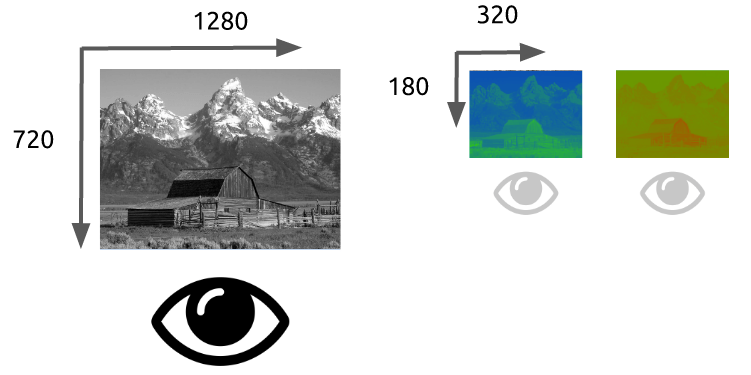
\includegraphics[width=0.8\textwidth]{img/rozdzial2/ycbcr_subsampling_resolution}
    \caption{}
    \caption[Prezentacja działania chroma subsampling]{Prezentacja działania chroma subsampling. Źródło: repozytorium digital-video-introduction}
    \label{fig:chroma_subsampling_resolution}
\end{figure}

\begin{figure}[H]
    \centering
    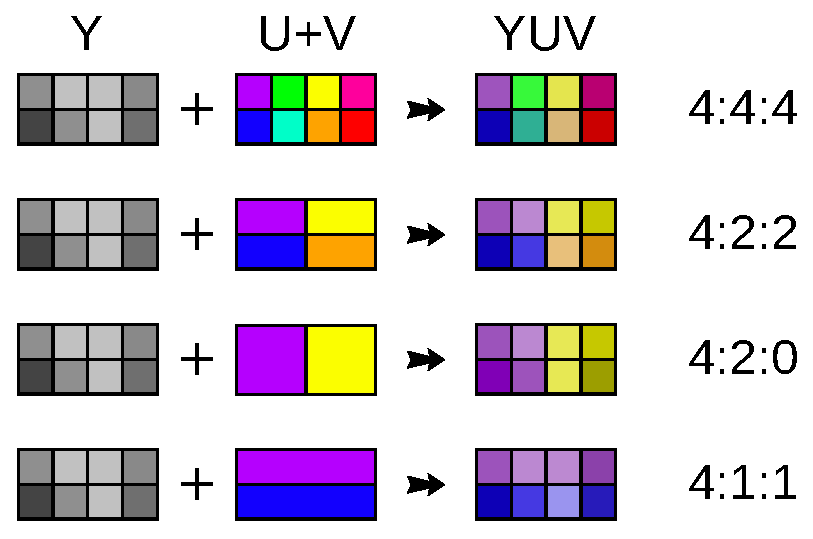
\includegraphics[width=0.6\textwidth]{img/rozdzial2/chroma_subsampling_ratios}
    \caption{Zasada działania różnych formatów chroma subsampling}
    \label{fig:chroma_subsampling_ratios}
\end{figure}

Jak widać na obrazku \ref{fig:chroma_subsampling_comparison}, pomimo bardzo niskiego próbkowania
informacji o kolorze, w górnym rzędzie nie widać znaczących różnic pomiędzy pierwszym i ostanim
obrazkiem.

\begin{figure}[H]
    \centering
    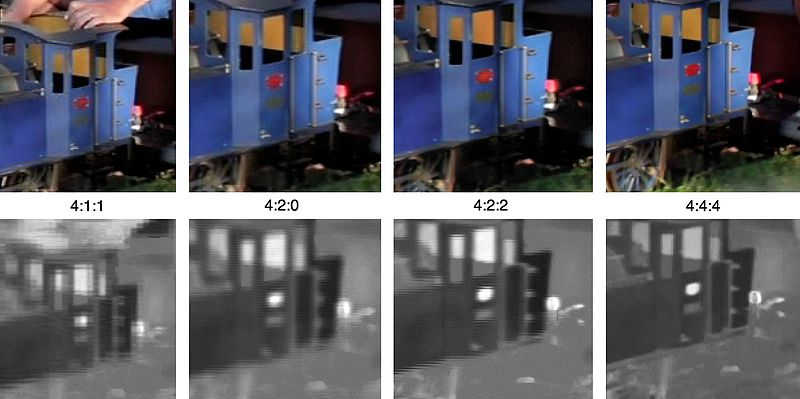
\includegraphics[width=\textwidth]{img/rozdzial2/chroma_subsampling_examples}
    \caption{Porównanie kanału chroma oraz rezultatu różnych formatów chroma subsampling}
    \label{fig:chroma_subsampling_comparison}
\end{figure}

\subsubsection{Kompensacja ruchu}

Kompensacja ruchu jest jedną z metod kompresji inter-frame, tzn. zmian pomiędzy klatkami. Ponieważ
często zawartość klatki zmienia się tylko częściowo, zostawiając inne elementy bez zmiany, możliwe
jest zapisanie tylko różnicy pomiędzy sąsiadującymi klatkami. Kompensacja ruchu usprawnia ten
proces: dzięki wprowadzeniu możliwości przenoszenia całych bloków, możemy zakodować zmiany w klatce
z użyciem mniejszej liczby bitów i zmniejszyć różnicę pomiędzy klatkami którą trzeba będzie
zaaplikować. Proces przezentuje kompensacja ruchu obiektu z rysunku \ref{fig:motion_compensation},
natomiast na rysunku \ref{fig:motion_compensation_residual} widoczna jest pozostała różnica po
procesie kompensacji.

\begin{figure}[H]
    \centering
    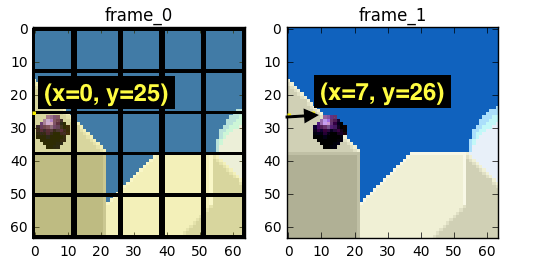
\includegraphics[width=.5\textwidth]{img/rozdzial2/original_frames_motion_estimation}
    \caption{Przykład sąsiadujących klatek na których występuje ruch}
    \label{fig:motion_compensation}
\end{figure}

\begin{figure}[H]
    \centering
    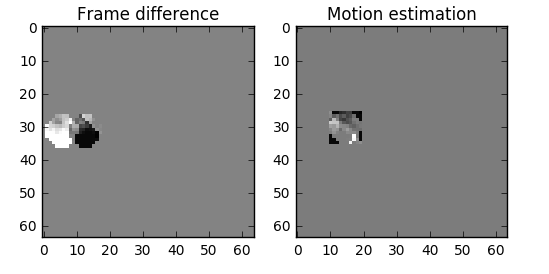
\includegraphics[width=.5\textwidth]{img/rozdzial2/difference_frames}
    \caption{Porównanie różnicy pomiędzy klatkami bez oraz z uwzględnieniem kompensacji ruchu}
    \label{fig:motion_compensation_residual}
\end{figure}

\subsubsection{Predykcja wewnątrzklatkowa}

Predykcja wewnątrzklatkowa (ang. intra-frame prediction) wykorzystuje redundancję w obrębie jednej
klatki do opisania jej z użyciem mniejszej liczby bitów. Widoczne na rysunku
\ref{fig:intra_frame_compression} oznaczone obszary zawierają obszary skorelowane, których wartości
mogą być przewidziane na podstawie wartości sąsiadujących pikseli.

\begin{figure}[H]
    \centering
    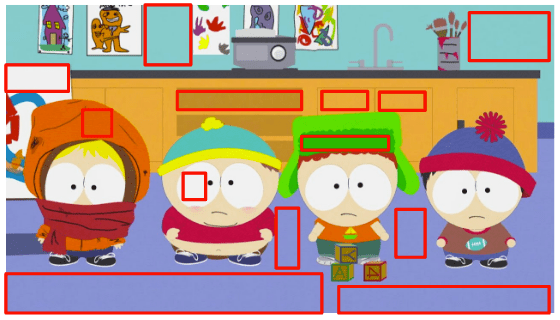
\includegraphics[width=.5\textwidth]{img/rozdzial2/repetitions_in_space}
    \caption{Klatka z serialu South Park z zaznaczonymi obszarami które można skompresować predykcją intra-frame}
    \label{fig:intra_frame_compression}
\end{figure}

\subsubsection{Dyskretna transformacja cosinusowa i kwantyzacja}

Uzyskany po zaaplikowaniu predykcji blok różnicy (ang. residual block) można następnie
przetransformować za pomocą DCT i następnie za pomocą kwantyzacji pozbyć się wyższych współczynników
przetransformowanego bloku. Proces przebiega podobnie jak DCT w kodowaniu JPG. Rysunki
\ref{fig:dct} oraz \ref{fig:quantization} przestawiają kolejno proces DCT oraz kwantyzacji (z
różnicą że podczas kwantyzacji nie dzieli się przez jedną wartość, tylko przez specjalne macierze kwantyzacji).

\begin{figure}[H]
    \centering
    \begin{subfigure}{0.48\linewidth}
        \centering
        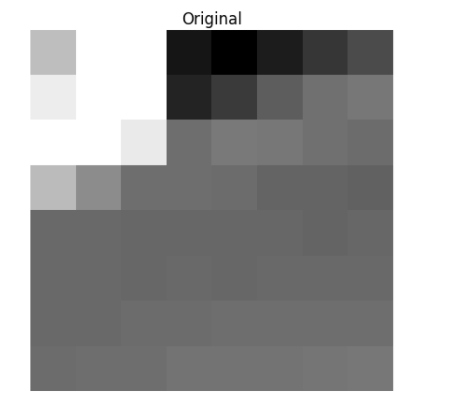
\includegraphics[width=.7\linewidth]{img/rozdzial2/dct_original}
        \caption{Blok różnicy po predykcji}
    \end{subfigure}
    \begin{subfigure}{0.48\linewidth}
        \centering
        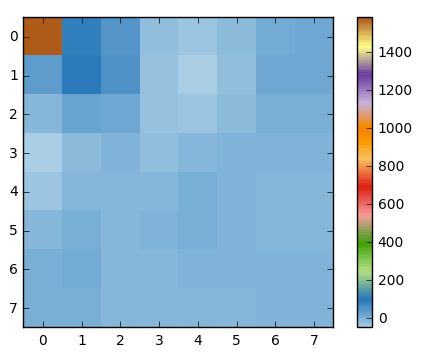
\includegraphics[width=.7\linewidth]{img/rozdzial2/dct_coefficients}
        \caption{Blok współczynników po DCT}
    \end{subfigure}
    \caption{Proces DCT}
    \label{fig:dct}
\end{figure}

\begin{figure}[H]
    \centering
    \begin{subfigure}{0.48\linewidth}
        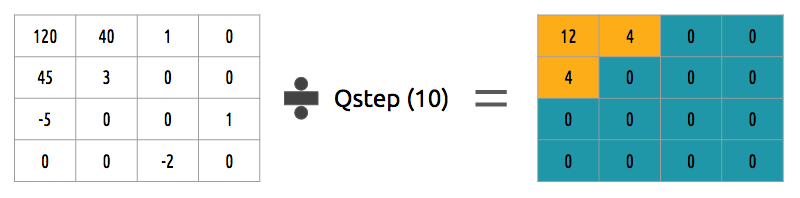
\includegraphics[width=.9\linewidth]{img/rozdzial2/quantization_1}
    \end{subfigure}
    \begin{subfigure}{0.48\linewidth}
        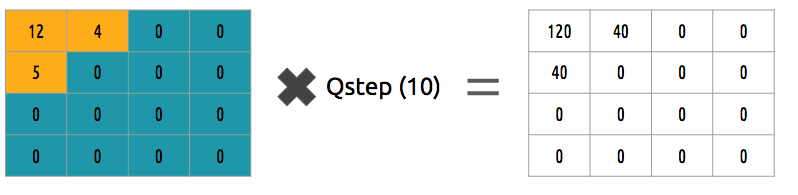
\includegraphics[width=.9\linewidth]{img/rozdzial2/quantization_2}
    \end{subfigure}
    \caption{Proces kwantyzacji}
    \label{fig:quantization}
\end{figure}

\subsubsection{Kodowanie entropijne}

Po kwantyzacji, ostatnim krokiem jest bezstratne skompresowanie powstałej sekwencji współczynników.
Można do tego celu wykorzystać różne sposoby kompresji bezstratnej, np. kodowanie Huffmana lub
kodowanie arytmetyczne.

% \subsection{AVC}

% AVC jest standardem kodowania wideo przyjętym w roku 2003 przez MPEG. Jego najpopularniejszą
% implementacją jest biblioteka x264.

% \subsection{AV1}
% \subsubsection{Partitioning}

% Klatka dzielona jest na sąsiadujące ze sobą tzw. superbloki, mające rozmiar 128x128 lub 64x64
% pikseli, które mogą być następnie podzielone na mniejsze bloki według pewnych wzorców. Wzorzec
% dzielący blok na bloki 2x2 równej wielkości pozwala na rekurencyjne dzielenie w coraz mniejsze
% bloki, aż do rozmiaru bloku 4x4 piksele.

% \begin{figure}[H]
%     \centering
%     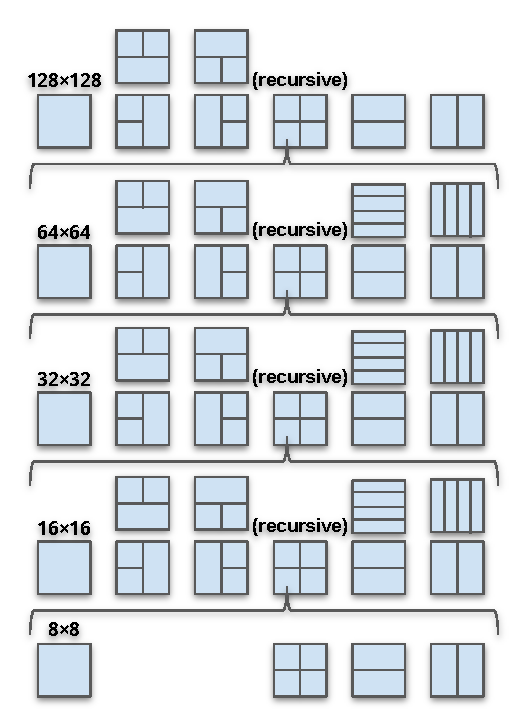
\includegraphics[width=.4\textwidth]{img/rozdzial2/av1_partitioning}
%     \caption{Diagram prezentujący wszystkie sposoby podzielenia bloków w AV1}
%     \label{fig:av1_blocks}
% \end{figure}


\section{Internetowe strumienie wideo}

Strumienie wideo w zależności od źródła mogą mieć różne charakterystyki i ograniczenia.
Możemy wyróżnić 3 rodzaje strumieni wideo:

\begin{itemize}
    \item lokalne pliki wideo - pliki wideo na dysku w kontenerze mp4, mkv, lub innym
    \item strumieniowanie plików wideo (np. Youtube albo Netflix) - przygotowane segmenty pliku
          wideo w różnych rozdzielczościach wysyłane są po kolei, rozdzielczość dobierana jest wg.
          dostępnego pasma pomiędzy serwerem a klientem
    \item strumieniowanie w czasie rzeczywistym - priorytetem jest opóźnienie, przechwytywane klatki
          kodowane są na bieżąco i są wysyłane najszybciej jak to możliwe; przez to niektóre
          mechanizmy kompresji są niedostępne (np. B-klatki, które wykorzystują dane z następnej
          klatki aby zmniejszyć wielkość klatki). O tych strumieniach jest mowa w pracy.
\end{itemize}

Zidealizowany obraz rozmowy wideo w internecie wygląda następująco:

\begin{enumerate}
    \item Komputery są publicznymi hostami w internecie i program komunikatora słucha na danym porcie
    \item Strona nawiązująca połączenie łączy się do hosta odbiorcy po tym porcie, sygnalizuje chęć
          nawiązania połączenia
    \item Strona odbierająca akceptuje
    \item Kamera oraz mikrofon nadawcy przechwytują najlepszy możliwy obraz i dźwięk, i przesyłają
          je do komputera
    \item Strumienie wideo i audio są łączone i synchronizowane
    \item Komputer wysyła strumień audio-wideo wcześniej ustanowionym kanałem
\end{enumerate}

Natomiast pojawiają się problemy:

\begin{enumerate}
    \item Komputery znajdują się w sieciach domowych, za NATem, nie można się do nich bezpośrednio
          połączyć
    \item Nieskompresowane wideo jest zbyt duże by wysłać je przez internet, potrzebny jest jakiś
          mechanizm kompresji
    \item Komputery mogą mieć różne możliwości przetwarzania wideo: znajdować się w sieciach o
          znacząco różnej szybkości, mieć różniące się szybkością procesory, kamery zapisujące
          klatki w różnych formatach
\end{enumerate}

\section{Wykorzystane technologie}

W tej sekcji zostaną opisane technologie użyte w dalszej części pracy.

\subsection{WebRTC}

Niniejszy rozdział przytacza fragmenty książki \emph{High Performance Browser Networking}
\cite{hpbn} celem opisu projektu WebRTC.

WebRTC jest standardem zapewniającym przeglądarkom możliwości komunikacji peer-to-peer w czasie
rzeczywistym, dzięki czemu możliwe jest budowanie komunikatorów internetowych w całości w obrębie
zapewnianego przez przeglądarkę javascriptowego API. Aby funkcjonalność ta była możliwa do
zrealizowania, niezbędne było użycie wielu protokołów sieciowych, które pokazano na rysunku
\ref{fig:webrtc_stack}.

\begin{figure}[htbp]
    \centering
    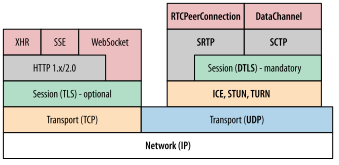
\includegraphics{img/webrtc-stack_hpbn}
    \caption{Stos protokołów w WebRTC}
    \label{fig:webrtc_stack}
\end{figure}

Głównym targetem WebRTC są przeglądarki, jednak istnieją także implementacje dla innych typów
aplikacji. W podrozdziale \ref{gstreamer_webrtc} opisano implementację dla frameworka GStreamer.

WebRTC pomaga rozwiązać 3 problemy niezbędne do nawiązania multimedialnego połączenia peer-to-peer:

\begin{enumerate}
    \item W jaki sposób zasygnalizować peerowi chęć nawiązania połączenia tak by zaczął on
          nasłuchiwać na wysyłane do niego dane?
    \item Jak wynegocjować odpowiednie parametry strumieni multimedialnych tak by odpowiadały one
          obu stronom?
    \item Jak zidentyfikować potencjalne trasy/tryby połączenia dla obu jego stron?
\end{enumerate}

\subsubsection{Sygnalizacja nawiązania połączenia}

Przed nawiązaniem komunikacji P2P i negocjacji parametrów strumieni mediów, należy najpierw
powiadomić drugą stronę połączenia o intencji nawiązania połączenia oraz ustalić czy peer jest
osiągalny. Ponieważ peer nie nasłuchuje jeszcze pakietów, potrzebny jest wspólny kanał
sygnalizacyjny przez który możliwa będzie sygnalizacja połączenia.

\begin{figure}[H]
    \centering
    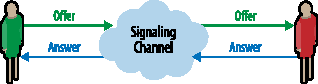
\includegraphics{img/signaling-1}
    \caption{Strony sygnalizacji}
    \label{fig:signaling}
\end{figure}

WebRTC nie wymusza żadnego protokołu transportowego do celów sygnalizacji, zamiast tego
pozostawiając wybór aplikacji. Pozwala to na interoperacyjność z istniejącymi już protokołami i
infrastrukturą.

W wypadku naszej aplikacji, rola kanału sygnalizacyjnego będzie pełniona przez serwer aplikacji.

\subsubsection{Negocjacja parametrów połączenia}
\label{negotiation}

WebRTC używa protokołu SDP (ang. Session Description Protocol) do opisu parametrów połączenia P2P.
Samo SDP nie zawiera żadnych mediów, zamiast tego opisuje tylko profil sesji, tj. zawiera listę
różnych właściwości połączenia, takich jak rodzaje strumieni, użyte kodeki i ich ustawienia,
prędkość transmisji, etc.

Aby ustanowić połączenie P2P, oba peery muszą wymienić swoje opisy SDP w procesie widocznym na
rysunku \ref{fig:signaling2}.

\begin{figure}[H]
    \centering
    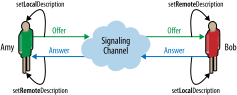
\includegraphics{img/signaling-2}
    \caption{Proces negocjacji}
    \label{fig:signaling2}
\end{figure}

\begin{enumerate}
    \item Strona inicjująca (Amy) rejestruje swoje lokalne strumienie mediów, tworzy z nich ofertę
          połączenia i ustawia ją jako lokalny opis sesji.
    \item Amy następnie wysyła wygenerowaną ofertę do drugiej strony połączenia (Bob).
    \item Gdy Bob otrzyma ofertę, ustawia on otrzymany opis sesji jako opis zdalny po swojej
          stronie, następnie rejestruje swoje strumienie, generuje z nich odpowiedź i ustawia ją jako
          lokalny opis sesji.
    \item Bob następnie wysyła swoją odpowiedź do Amy.
    \item Gdy Amy otrzyma odpowiedź od Boba, ustawia ona tą odpowiedź jako zdalny opis sesji.
\end{enumerate}

Po zakończeniu procesu wymiany opisów sesji przez kanał sygnalizacyjny, obie strony połączenia
wynegocjowały jego parametry i ustawienia. Ostatnim krokiem jest nawiązanie połączenia P2P.

\subsubsection{Interactive Connectivity Establishment (ICE)}
\label{ice}

By możliwe było nawiązanie połączenia P2P, oba peery powinny muszą być w stanie trasować pakiety do
siebie nawzajem. Niestety istnieje wiele przeszkód mogących to uniemożliwić, np. NAT lub firewalle.
Jeżeli oba peery znajdują się w tej samej sieci lokalnej, każdy peer może po prostu wysłać drugiej
stronie swój adres IP w sieci lokalnej. Co jednak w sytuacji gdy peery znajdują się w różnych
sieciach? Peery musiałyby wtedy znaleźć swój publiczny IP oraz w jakiś sposób otworzyć NAT na ruch
od drugiej strony połączenia.

Na szczęście WebRTC również pomaga w tym aspekcie nawiązywania połączenia. Robi to za pomocą
mechanizmu ICE (Interactive Connectivity Establishment).

\begin{itemize}
    \item Każda strona połączenia zawiera agenta ICE
    \item agent ICE jest odpowiedzialny za znajdywanie adresów IP oraz numerów portów (kandydatów)
    \item agent ICE jest odpowiedzialny za sprawdzanie połączeń pomiędzy stronami
    \item agent ICE jest odpowiedzialny za podtrzymywanie połączenia
\end{itemize}

Gdy opis sesji zostanie ustawiony, lokalny agent ICE rozpoczyna proces odkrywania wszystkich
możliwych adresów pod którym możliwe jest połączenie z lokalnym peerem

\begin{enumerate}
    \item agent ICE pyta system operacyjny o lokalny adres IP
    \item Jeśli istnieje, agent ICE pyta zdalny serwer STUN o publiczny adres IP i numer portu
          lokalnego peera.
    \item Jeśli istnieje, agent ICE wykorzystuje serwer TURN jako pośrednik do ruchu pomiędzy
          peerami jeżeli niemożliwe jest ustanowienie połączenia P2P z powodu np. zbyt restrykcyjnego NATa.
\end{enumerate}

Powyższe procesy są wykonywane automatycznie, w tle, programista musi tylko w odpowiedni sposób
obsłużyć zdarzenia generowania i otrzymywania kandydatów ICE.

\subsection{GStreamer}

GStreamer jest frameworkiem do tworzenia strumieniujących aplikacji multimedialnych
\cite{gstreamer}. Aplikacje są wyrażane jako "rurociąg" składający się z bloków. Rdzeń GStreamer
definiuje architekturę aplikacji oraz API dla elementów, a same elementy są zawarte w różnych
pluginach. Jego modularna architektura sprawia że nie jest ograniczony do aplikacji audio-wideo,
lecz może być wykorzystany do każdej aplikacji, która strumieniowo przetwarza dowolne rodzaje
danych.

\begin{figure}[H]
    \centering
    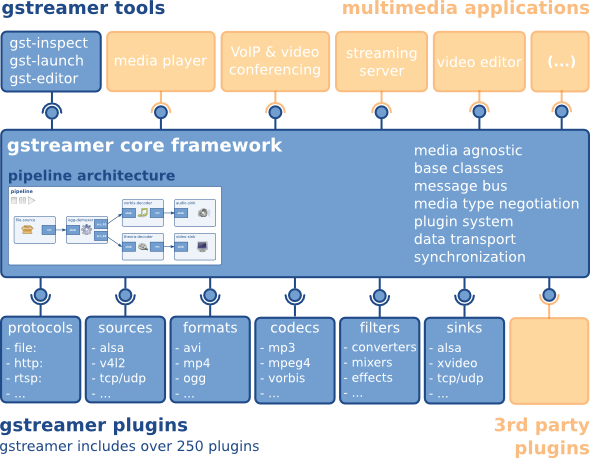
\includegraphics[width=.5\textwidth]{img/technologie/gstreamer-overview}
    \caption{Architektura projektu GStreamer}
\end{figure}

Dane generowane są elementach-źródłach (source), są przetwarzane przez elementy-filtry (filter), a
następnie są konsumowane w elementach-zlewach (sinks). Elementy są częścią rurociągu, który w danym
czasie może być zatrzymany, zapauzowany, lub uruchomiony. Zmiana stanu rurociągu zmienia stan
wszystkich jego elementów.

\begin{figure}[H]
    \centering
    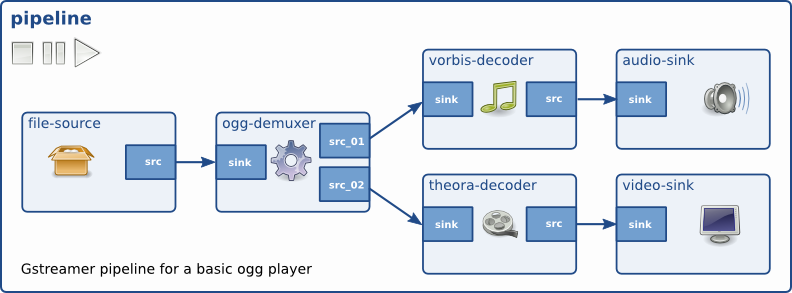
\includegraphics[width=.7\textwidth]{img/technologie/simple-player}
    \caption{Przykładowy rurociąg aplikacji GStreamer}
    \label{fig:gstreamer_example_pipeline}
\end{figure}

Rysunek \ref{fig:gstreamer_example_pipeline} przedstawia rurociąg przykładowego odtwarzacza plików
OGG. Dane przechodzą przez rurociąg od lewej do prawej strony, będąc transformowane w każdym
elemencie.

\subsubsection{GStreamer WebRTC}
\label{gstreamer_webrtc}

GStreamer posiada swoją własną implementację WebRTC, wykonaną przez firmę Centricular. Jej głównym
elementem jest element
\href{https://gstreamer.freedesktop.org/documentation/webrtc/index.html?gi-language=c}{webrtcbin}.
Ten element zajmuje się procesami negocjacji parametrów połączenia oraz zbierania i udostępniania
kandydatów ICE omówionymi w podrozdziałach \ref{negotiation} i \ref{ice}. Zdarzenia takie jak
pojawienie się nowego strumienia multimedialnego są komunikowane aplikacji za pomocą sygnałów, które
są obsługiwane zazwyczaj poprzez tworzenie nowych elementów i dodanie ich do rurociągu celem
prezentacji przychodzącego strumienia użytkownikowi.

\subsection{GTK4 i libadwaita}

Do wykonania aplikacji graficznej wykorzystany został darmowy, otwartoźródłowy, wieloplatformowy
framework GTK4 oraz biblioteka libadwaita implementująca często wykorzystywane komponenty i wzorce
projektowe będące częścią wytycznych projektu GNOME w projektowaniu interfejsów
(\href{https://developer.gnome.org/hig/}{GNOME Human Interface Guidelines}).

GTK jest najpopularniejszą biblioteką używaną do tworzenia graficznych aplikacji dla systemów Linux.
Napisana w C, wykorzystuje jednak paradygmat obiektowy; używa biblioteki GObject która zapewnia
system klas i obiektów, a także inne zależności widoczne na rysunku \ref{fig:gtk_toolkit}.

\begin{figure}[H]
    \centering
    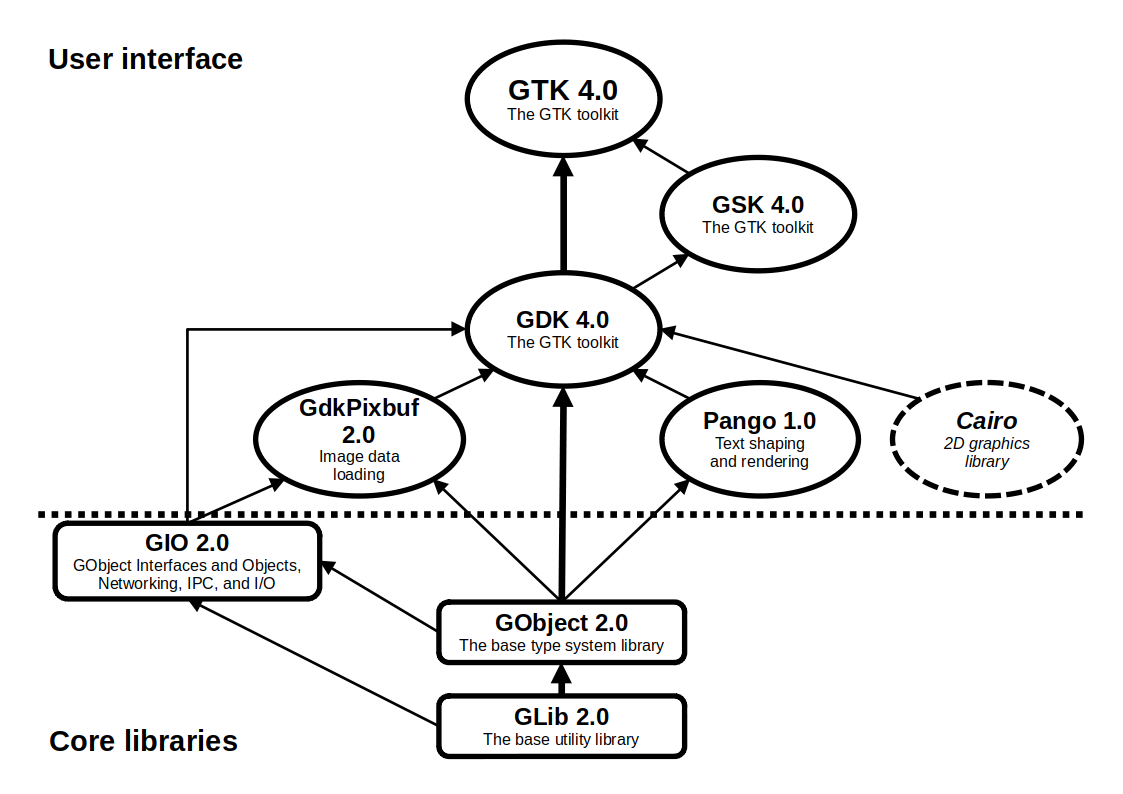
\includegraphics[width=.7\textwidth]{img/gtk-toolkit}
    \caption{Architektura zestawu narzędzi GTK}
    \label{fig:gtk_toolkit}
\end{figure}

Bezpośrednie używanie tych bibliotek w języku Rust nie jest jednak rekomendowane, i gdzie tylko
możliwe wykorzystywane są biblioteki natywne dla języka Rust. Nie można ich jednak wyeliminować lub
zastąpić, ponieważ są twardymi zależnościami frameworka GUI.

Pomimo tego, GTK zostało wybrane z dwóch powodów:

\begin{itemize}
    \item GTK jest najpopularniejszym, najbardziej sprawdzonym oraz dojrzałym frameworkiem GUI dla
          systemów Linux
    \item GStreamer i GTK są częściami tego samego projektu freedesktop i w związku z tym
          interoperują ze sobą; m.in. wykorzystują te same biblioteki GLib i GObject, a także
          GStreamer może rysować zawartość strumienia mediów na powierzchnię jeżeli ta
          implementuje interfejs \verb|GstVideoOverlay|.
\end{itemize}

\subsection{Rust}

Rust jest językiem programowania generalnego zastosowania rozwijanym przez fundację Mozilla.
Stworzony z myślą o bezpieczeństwie, współbieżności, i praktyczności, zapewnia wydajność bliską
języka C jednocześnie gwarantując bezpieczeństwo pamięci nie wykorzystując przy tym mechanizmu
Garbage Collection. Zamiast tego Rust wykorzystuje "borrow checker", który śledzi czas życia
referencji do obiektów podczas kompilacji. Dzięki temu niektóre klasy błędów są niemożliwe do
popełnienia, dzięki czemu programista może wykorzystywać wielowątkowość bez obaw przed ezoterycznymi
i nietrywialnymi do zdebugowania błędami typu race-condition. Ponadto dzięki darmowym abstrakcjom,
kod w języku Rust jest czytelny jak język wysokopoziomowy, jednocześnie zapewniając wydajność
charakterystyczną zazwyczaj tylko dla języków niskopoziomowych.

\subsection{Programowanie asynchroniczne}

Programowanie asynchroniczne jest paradygmatem programowania umożliwiającym konkurentne wykonywanie
wielu zadań bez użycia mechanizmów wielowątkowości. Zamiast tego, główny wątek programu może zapisać
stan aktualnie wykonywanego zadania i zająć się wykonywaniem innego zadania. Paradygmat ten
jest popularny przy programowaniu serwerów, ponieważ wielowątkowość charakteryzowała się wieloma
wadami:

\begin{itemize}
    \item Wątki są powolne do tworzenia, i zajmują pewną minimalną ilość pamięci - zadania
          asynchroniczne można tworzyć bardzo szybko i zajmują one o wiele mniej pamięci
    \item Użycie wielu wątków może prowadzić do błędów typu race-condition - zadania
          asynchroniczne mogą być przypisane do jednego wątku eliminując ten problem
    \item Jeżeli używana jest bardzo duża liczba wątków, overhead systemu operacyjnego staje się
          znaczący i wydajność systemu może ucierpieć - w systemie asynchronicznym planowanie
          zadań jest prostsze ponieważ dzieje się w userspace przez egzekutor systemu
          asynchronicznego, nie występują zatem drogie context-switche, a także egzekutor lepiej
          zna charakterystyki wykonywanego kodu więc może planować tak by zużycie zasobów było
          mniejsze
    \item Większość sytuacji wymagających konkurentności w serwerach to czekanie na jakieś
          zdarzenie: czekanie na połączenie, czekanie na odebranie danych od klienta, etc. tzw.
          IO-bound. W takiej sytuacji nie ma potrzeby zwiększać złożoności systemu angażując
          kolejne fizyczne procesory i pamięć, zamiast tego wątek może w tym czasie pracować nad
          innymi zadaniami.
\end{itemize}

Ekosystem programowania asynchronicznego składa się z asynchronicznych tzw. runtimes zawierających
egzekutory zadań asynchronicznych oraz samych zadań asynchronicznych znanych jako Futures. Future
(ang. przyszłość) reprezentuje operacje która zwróci wartość w przyszłości i musi być w tym celu
możliwie wielokrotnie wykonywana funkcją \verb|poll()|, która może zwrócić wariant
\verb|Poll::Ready(T)| reprezentujący zakończenie działania i zwrócenie wartości, lub wariant
\verb|Poll::Pending| wskazujący że wykonany został pewien postęp w wykonaniu, jednak funkcja będzie
musiała zostać wykonana ponownie.

Sam egzekutor wykorzystuje asynchroniczne system calle takie jak epoll, które sprawiają że gdy
wydarzy się zdarzenie, w kontekście future wywołuje się funkcja \verb|wake()|, która powiadamia
egzekutor o tym że dana future może być pollnięta ponownie.

Overhead takiego podejścia jest mały i działa ono bardzo dobrze, dopóki futures są IO-bound, tj.
większość czasu to czas spędzony na czekanie na IO. Gdy futures są CPU-bound, tj. wykonują dużą
ilość kalkulacji których zakończenie zajmie znaczącą ilość czasu (np. kilka sekund), lub używają
synchronicznych blokujących API, wtedy taka future jest w stanie zablokować egzekutor i inne futures
nie będą w stanie się wykonać. W tym celu asynchroniczne runtimes zazwyczaj udostępniają specjalny
thread pool na zadania blokujące główny wątek. Dodatkowo, egzekutor zazwyczaj też wykorzystuje
thread pool do uruchamiania futures, dzięki czemu mogą być one wykonywane nie tylko współbieżnie lecz
także równolegle. Dzięki gwarancjom bezpieczeństwa i systemowi ownership w języku Rust, nie powoduje
to ryzyka wystąpienia błędów związanych z wielowątkowością. To czy future może zostać wysłana
pomiędzy wątkami jest wiadome już w procesie kompilacji, dzięki traitowi \verb|Send|. Funkcje
egzekutorów typu \verb|task::spawn()| służące do rozpoczęcia współbieżnego wykonania danego future
wymagają aby była ona \verb|Send|, a jeżeli nie jest, emitowany jest błąd kompilacji. Istnieją także
funkcje jak \verb|task::block_on()| które synchronicznie wykonują dany future na jednym wątku.

W niniejszym projekcie gdy tylko możliwe preferowane jest używanie asynchronicznych API.
Wykorzystywane są oba najpopularniejsze runtime'y asynchroniczne w języku Rust: tokio oraz
async-std.
